\section{RQ1: What Does Exact Deletion Do?}\label{sec:rq1}

This section compares the reference model of Section~\ref{sec:exp},
trained on the full five-year window, with the oracle, retrained
after one training year is removed. The comparison produces two
quantities, measured on different parts of the data.

The memorization gap $G$ (Eq.~\ref{eq:gap}) is measured on the
removed year. It is the oracle's forecast error on that year minus
the reference's error on the same year. The reference trained on the
year and the oracle did not, so a large gap means that fitting the
year required training on it. $G$ therefore measures how much of the
year the model memorized.

The deletion effect $\Delta$ (Eq.~\ref{eq:delta}) is measured on the
test year. It is the oracle's forecast skill minus the reference's
skill. Neither model trained on the test year, so $\Delta$ measures
what the deletion does to subsequent forecasts. A positive $\Delta$
means the model forecasts better without the removed year. We report
$G$ first, then $\Delta$, and finally how both depend on which year
of the window is removed.

Tables~\ref{tab:years} and~\ref{tab:skill} provide the context for
these results. Table~\ref{tab:years} summarizes the market conditions
of each year. The COVID crisis year 2020 is by far the most volatile
year in the sample, with $38\%$ realized volatility, compared with
$24\%$ in the 2022 bear market and $7$--$18\%$ in the low- to
medium-volatility years.
Table~\ref{tab:skill} reports the test skill of the five
architectures. The deployable models, the Transformer, TSMixer, and
SegRNN, exceed the HAR benchmark in every fold. The non-deployable
models, iTransformer and PatchTST, never do. Both distinctions, the
crisis year against the low- to medium-volatility years and the
deployable models against the non-deployable ones, recur throughout
the results.

\begin{table}[t]
\caption{Realized volatility of the deletable years
(equal-weighted panel); each sits inside at least one training
window. 2020 is the COVID crisis, 2022 the bear market, and the
remaining years are low- to medium-volatility years. The test
years' volatilities appear with the fold results.}
\label{tab:years}
\centering
\setlength{\tabcolsep}{3.6pt}
\footnotesize
\begin{tabular}{lcccccccc}
\toprule
Year & 2016 & 2017 & 2018 & 2019 & \textbf{2020} & 2021 & 2022 & 2023\\
\midrule
Realized vol.\ (\%) & 14 & 7 & 16 & 13 & $\mathbf{38}$ & 14 & 24 & 14\\
\bottomrule
\end{tabular}
\end{table}

\begin{table}[t]
\caption{Reference skill (IC) per fold. Rows are sorted by skill,
and the refitted HAR benchmark, evaluated on the same test years,
separates the deployable models above it from the non-deployable
models below it. Folds are ordered by test-year volatility.}
\label{tab:skill}
\centering
\setlength{\tabcolsep}{5pt}
\footnotesize
\begin{tabular}{lcccc}
\toprule
& 2022 & 2025 & 2023 & 2024\\
Architecture & ($24\%$) & ($18\%$) & ($14\%$) & ($12\%$)\\
\midrule
Transformer & $0.570$ & $0.454$ & $0.470$ & $0.489$\\
TSMixer & $0.560$ & $0.463$ & $0.458$ & $0.488$\\
SegRNN & $0.517$ & $0.452$ & $0.441$ & $0.476$\\
\midrule
HAR (benchmark) & $0.508$ & $0.412$ & $0.384$ & $0.396$\\
\midrule
iTransformer & $0.125$ & $0.213$ & $0.174$ & $0.221$\\
PatchTST & $0.168$ & $0.181$ & $0.181$ & $0.169$\\
\bottomrule
\end{tabular}
\end{table}

\begin{figure}[t]
\centering
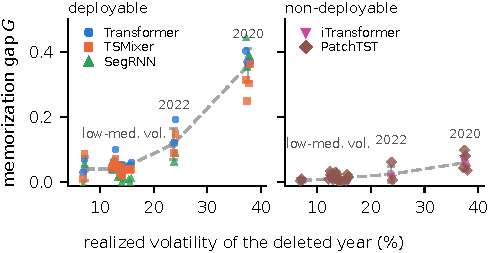
\includegraphics[width=0.92\columnwidth]{figs/fig_gap}
\caption{Memorization gap $G$ for all 100 cells (5 architectures
$\times$ 4 folds $\times$ 5 deleted years, \Lone; each point the
mean of 10 seeds), placed at the realized volatility of the deleted
year and jittered horizontally by fold. Left: the three deployable
architectures. Right: the two non-deployable ones, on the same
vertical scale. The grey dashed curve connects the means of the
four volatility clusters, bars $\pm 1$ sd.}
\label{fig:gap}
\end{figure}

\subsection{Memorization of training years}

Figure~\ref{fig:gap} shows the memorization gap for every combination
of architecture, fold, and deleted year. Each point is placed at the
realized volatility of the deleted year. The gap increases with
volatility for every architecture. Deleting 2020 produces the largest
gap in every fold, the low- to medium-volatility years produce gaps
near zero, and the 2022 bear year lies between the two. Models therefore memorize
volatile years far more strongly than calm ones.

The size of the gap depends on model capacity. For every deleted
year, the three deployable architectures (left panel) show
gaps several times larger than the two non-deployable ones (right
panel). The
HAR benchmark shows the same pattern at a much smaller magnitude. The
volatility of a year determines whether it is memorized, and model
capacity determines how strongly.

A plausible explanation is the absence of substitutes. A model
trained without 2019 can still fit 2019, because the remaining calm
years contain similar dynamics. A model trained without 2020 cannot
reconstruct the crisis from the remaining years, because none of them
resembles it. Two controls support this interpretation. A placebo
deletion that removes the same number of training windows at random
produces no gap, and the gap is unrelated to how well the reference
model fits each year. The gap therefore reflects the content of the
deleted year, not the amount of data removed and not the difficulty
of the year.

\begin{figure}[t]
\centering
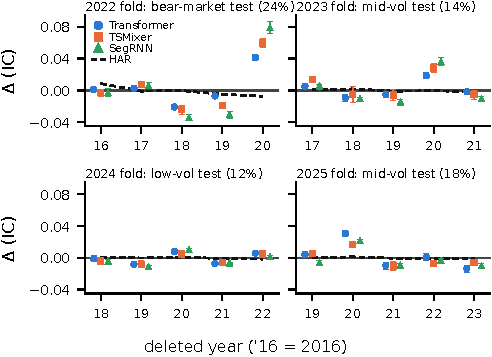
\includegraphics[width=0.92\columnwidth]{figs/fig_ladder}
\caption{Deletion effect $\Delta$ of removing each training year,
in every fold (\Lone, 10 seeds per point, bars $\pm 1$ standard
error; all panels share one scale; points offset slightly for
visibility). The dashed black line is the refitted HAR benchmark.
The two non-deployable architectures share no common shape and are
omitted.}
\label{fig:ladder}
\end{figure}

\subsection{Effect of deletion on forecast skill}

Figure~\ref{fig:ladder} reports the deletion effect for the three
deployable architectures. Each panel corresponds to one
fold, and each point gives the change in test-year skill caused by
deleting one training year. A positive value means that the model
forecasts better without that year. Deleting 2020 improves all three
architectures in all four folds. The improvement is largest in the
2022 fold, whose bear-market test year is most similar to the
deleted crisis, and it decreases as the test year becomes calmer. In
the 2024 fold, which has the lowest-volatility test year, no
architecture
changes by more than about $3\%$ of its skill, an amount close to
the placebo effect. The most strongly memorized year is therefore
also the only year whose deletion consistently improves forecasts.

If the 2020 observations were simply misleading about later markets,
every model should improve when they are removed. The HAR benchmark,
subjected to the identical deletion (dashed line in each panel),
instead loses a small amount of skill. The benchmark has too little
capacity to memorize the crisis and extracts useful information from
the 2020 data. The improvement therefore reflects a property of the
deployable models, not a defect of the data. Prior work shows
that memorizing atypical examples improves test accuracy when
training and test distributions
coincide~\cite{feldman2020memorization}. In our setting the test
regime differs from the memorized one, and memorization reduces
accuracy instead. The data cannot identify which property of the
deployable models drives the improvement, because test skill and
memorization increase together across the five architectures. The
effect is not specific to a single architecture. TSMixer was added
after the experimental design was fixed, its improvement under the
2020 deletion was predicted in advance, and the prediction was
confirmed.

The two non-deployable architectures show no comparable
regularity. Their deletion effects change sign across folds and
deletion levels, and PatchTST loses about $40\%$ of its skill in the
bear-market fold. The HAR benchmark therefore also functions as a
screening criterion. The deployable models respond to deletion
consistently, and the non-deployable models do not. The gains
are also not carried by a few turbulent days. The oracle
outperforms the reference on the majority of individual test days.

\subsection{Dependence on the position of the deleted year}

Comparing the five deletions within each panel of
Figure~\ref{fig:ladder} shows that the position of the deleted year
matters. Deleting the earliest years of a window has almost no
effect. Deleting the low- to medium-volatility years immediately
before the test period reduces skill. Deleting the crisis year improves skill at
every position in the window. As the window slides forward, this
pattern moves with it.

We do not have a complete explanation for this pattern. The most
natural hypothesis is that a deletion helps when it makes the
training distribution more similar to the test year. The data
contradict it. The 2020 deletion shifts the training distribution
furthest from the test year, yet it is the only deletion that helps.
The results support two more limited conclusions. Recent low- to
medium-volatility years contain information that the models still
use, and a crisis year can degrade a high-capacity model once its
regime has passed.
Both effects are present within a single training window, and which
one a given deletion produces cannot be predicted from the data
alone. The retraining oracle measures it directly.

\subsection{Dependence on the deletion level}\label{sec:levels}

\begin{table}[t]
\caption{Price and measurement at each deletion level. Each
stricter reading of ``delete 2020'' is measured against its own
oracles. Data cost is the share of training windows surrendered,
$G(2020)$ is the memorization gap of the Transformer averaged over
folds and seeds, and the last column is the delete-2020 effect
across the twelve deployable cells. \Lone{} is the paper-wide
default.}
\label{tab:levels}
\centering
\footnotesize
\begin{tabular}{llcc}
\toprule
Level & Data cost & $G(2020)$ & Delete-2020 effect \\
\midrule
\Lzero & $20\%$ of windows & $0.527$ & $12/12$, all significant \\
\Lone & $+25\%$ windows & $0.375$ & $12/12$, all significant \\
\Ltwo & a further $+2\%$ & $0.368$ & $12/12$, $11$ significant \\
\bottomrule
\end{tabular}
\end{table}

Every result so far reads the deletion request at \Lone. The grid
repeats each deletion at \Lzero{} and \Ltwo{} with the same ten
seeds, so the price of strictness is measured rather than assumed.
Table~\ref{tab:levels} summarizes what the level changes.

Measured memory moves most. The crisis-year gap falls at each
stricter reading, in all twenty architecture-fold cells. The forget
sets are nested, so this decline means the windows each stricter
level adds carry smaller gaps than the crisis core. Nearly all of
the decline occurs in the step from \Lzero{} to \Lone, the step
that adds the overlapping context windows and recomputes
normalization. The further step to \Ltwo{} barely moves the gap. The gaps of the
low- to medium-volatility years move by less and in directions that
depend on the year. Two contracts naming the same period at
different levels therefore measure different amounts of memory.

No conclusion of this section changes direction with the level.
Deleting 2020 helps every deployable architecture at every level,
in all twelve cells, and only at \Ltwo{} does one cell lose
statistical significance. The losses from deleting the years just
before the test period are confirmed at \Lzero{} in the bear-market
fold, so they are not an artifact of the wider \Lone{} forget set.
The non-deployable models are not even stable across readings.
iTransformer's delete-2020 effect is positive at \Lzero{} and
vanishes at \Lone. \Lthree{} coincides with \Ltwo{} by
construction. The deletion level is a genuine contract parameter.
It changes what a deletion costs and how much memory it measures,
but not the direction of any finding. RQ2 asks whether retraining,
at whatever level the contract names, can be avoided.
